\documentclass[12pt]{article}
\usepackage{scrtime} % for \thistime (this package MUST be listed first!)
\usepackage[margin=0.75in]{geometry}
\usepackage{graphicx}
\usepackage{fancyhdr}
\usepackage{caption}
\usepackage{subcaption}
\usepackage{xspace}
%\usepackage{underscore}
\usepackage{pdfpages}
\usepackage{xcolor,colortbl}%for changing cell colour
\usepackage{longtable}
\usepackage{hyperref}
\usepackage{booktabs}
\pagestyle{fancy}
\setlength{\headheight}{15.2pt}
\setlength{\headsep}{13 pt}
\setlength{\parindent}{28 pt}
\setlength{\parskip}{12 pt}
\pagestyle{fancyplain}
\usepackage[T1]{fontenc}
\usepackage{tikz-cd}
\usepackage{tikz}
\usepackage[normalem]{ulem} %to strikeout text
\usetikzlibrary{decorations.markings}
\usetikzlibrary{calc, arrows}
\usepackage{lscape} %to make the page landscape
\usepackage{color,amsmath,amssymb,amsthm,mathrsfs,amsfonts,dsfont}
\usepackage{indentfirst} % to indent the first paragraph
\rhead{\fancyplain{}{Thesis Update \today \hfill Daniella Lato}}
%\rhead{\fancyplain{}{Thesis Update April 8, 2019 \hfill Daniella Lato}}
\title{Sinorhizobium Update}
\author{Daniella Lato}
\date{\today}
\renewcommand\headrulewidth{0.5mm}
\newcommand{\cc}{\cellcolor{black!16}}
\newcommand{\s}{\textit{Sinorhizobium}\xspace}
\newcommand{\smel}{\textit{S.\,meliloti}\xspace}
\newcommand{\smed}{\textit{S.\,medicae}\xspace}
\newcommand{\sfred}{\textit{S.\,fredii}\xspace}
\newcommand{\ssah}{\textit{S.\,saheli}\xspace}
\newcommand{\ster}{\textit{S.\,terangae}\xspace}
\newcommand{\agro}{\textit{A.\,tumefaciens}\xspace}
\newcommand{\escoli}{\textit{Escherichia coli}\xspace}
\newcommand{\bur}{\textit{Burkholderia}\xspace}
\newcommand{\vib}{\textit{Vibrio}\xspace}
\newcommand{\sul}{\textit{Sulfolobus}\xspace}
\newcommand{\ent}{\textit{Enterobacteria}\xspace}
\newcommand{\p}{progressiveMauve\xspace}
\newcommand{\bas}{\textit{Bacillus subtilis}\xspace}
\newcommand{\strep}{\textit{Streptomyces}\xspace}
\newcommand{\bass}{\textit{B.\,subtilis}\xspace}
\newcommand{\ecol}{\textit{E.\,coli}\xspace}
\newcommand{\ecoli}{\textit{Escherichia coli}\xspace}
\newcommand{\tub}{\textit{Mycobacterium tuberculosis}\xspace}
\newcommand{\pa}{pSymA\xspace}
\newcommand{\pb}{pSymB\xspace}
\newcommand{\snat}{\textit{S.\,natalensis}\xspace}
\newcommand{\scoe}{\textit{S.\,coelicolor}\xspace}
\newcommand{\borrb}{\textit{Borrelia burgdorferi}\xspace}
\providecommand{\e}[1]{\ensuremath{\times 10^{#1}}}
\newcommand{\ch}{$\checkmark$}
\newcommand{\dn}{\textit{dN}\xspace}
\newcommand{\ds}{\textit{dS}\xspace}
\newcommand{\sven}{\textit{S.\,venezuelae}\xspace}
%\newcommand{\scoe}{\textit{S.\,coelicolor}\xspace}
\newcommand{\sliv}{\textit{S.\,lividans}\xspace}
\newcommand{\bor}{\textit{Bordetella}\xspace}
\newcommand{\xan}{\textit{Xanthomonas}\xspace}
\begin{document}
%	Nov 30:	Create graphs with slopes for each COG
	
	
%	Dec 3:	Create new binned scatter plot of COG log reg
	
%	Dec 6:	Determine if there are any other stats I want/need for COG stuff
	
%	Dec 10:	Calculate above stats and write in table
	
%	Dec 21:	Find papers on COG stuff (for intro and discussion), and other mol trends (discussion for sub paper)
	
%	Jan 6:	Read above mentioned papers and make notes
%	Oct 31: Write out methods for gene expression paper
%	
%	Sep 9: Think about/compile list of inversions in \ecol for new paper
%	
%	Nov 15: Think about how to better look at the COG data
%	
%	Nov 25: Complete any extra analysis needed for Substitution paper
%	
%	Dec 4: Mac Scholarships and Awards Due
%	
%	Dec 1: Write out COG methods
%	
%	Dec 15: Gather papers for COG paper intro
%	
%	Dec 15: Implement COG stuff
%	
%	Other things to do:
%	
%	Create outline for gene expression paper
%
%  research mito increased subs near origin
%
%  add above to subs paper writeup
%	
%	Write Write Write gene expression paper
%	
%	 Have gene expression/inversion data combined and in graphical format/regression lines calculated
%	
%	re-do gene exp/sub graphs with patchwork R package so they line up exactly
%	
%	Have data for other molecular trends (GC content, number of genes, essential gene lists..etc.) combined with graphs (or in supplement) for sub analysis
%
% organize all the notes I made for comps into topics that can be integrated into an intro if needed
%	
%	May 31:	Complete COG analysis
%	
%	Jun 30:	COG analysis Paper draft completed
%	
%	Jul 31: Add other mol trends to Sub Paper

\underline{Subs Paper Things to Do:}
\begin{itemize}
	\item  \sout{more genomes}
	\item \sout{new  outgroups? (too distant)}
	\item \sout{explain high dS values in \bass}
	\item \sout{potentially poor alignment and non-orthologous genes (core genome, change methods?)}
	\item \sout{non-parametirc analysis for subs}
	\item \sout{gap in \ecoli fig 5}
	\item \sout{new methods for trees}
	\item \sout{concerned about repeated genes (TEs) and not analyzing core genome}
	\item \sout{check if trimming respects coding frame}
	\item \sout{clear distinction between mutations and substitutions in intro (separate sections)}
	\item \sout{datasets from previous papers (repeat my analysis on them?)}
	\item \sout{why would uncharacterized proteins have higher subs rates?}
	\item \sout{$R^2$ values in regression analysis}
	\item \sout{update gene exp paper ref}
	
%	\item \sout{ \# of coding and non-coding sites}
%	
%	\item \sout{\# of subs in each of $\uparrow$}
%	
%	\item \sout{Look into \strep non-coding issue}
%	
%	\item \sout{Look into \ecol coding issue}
%	
%	\item \sout{Look into \pb coding/non-coding trend weirdness}
%	
%	\item \sout{Figure out why \strep appears to have tons of coding data missing}
%	
%	\item \sout{Figure out what is going on with cod/non-cod code and why it is still not working!}
%	
%	\item \sout{write up methods for coding/non-coding}
%	
%	\item \sout{write methods and results for clustering}
%	
%	\item \sout{start code to split alignment into multiple alignments of each gene}
%	
%	\item \sout{figure out how to deal with overlapping genes}
%
%	\item \sout{figure out how to deal with gaps in gene of ref taxa}
%	
%	\item \sout{split up the alignment into multiple alignments of each gene}
%	
%	\item \sout{check if each gene alignment is a multiple of 3 (proper codon alignment)}
%	
%	\item \sout{get dN/dS for coding/non-coding stuff per gene}
%	 
%	\item Or get 1st, 2nd, 3rd codon pos log regs
	
%	\item \sout{write up coding/non-coding results}
%	
%	\item \sout{take out gene expression from this paper}
%	
%	\item \sout{write better intro/methods for distribution of subs graphs}
%	
%	\item \sout{write discussion for coding/non-coding}
%	
%	\item \sout{write coding/non-coding into conclusion}
%	
%	\item \sout{figured out pipeline for CODEML to calculate dN/dS for each gene}
%	
%	\item \sout{make a list of what should be in supplementary files for subs paper}
%	
%	\item \sout{put everything in list into supplementary file for subs paper}
%	
%	\item \sout{write dN/dS methods}
%	
%	\item \sout{write dN/dS results}
%	
%	\item \sout{write dN/dS discussion}
%	
%	\item \sout{write dN/dS into conclusion}
%	
%	\item \sout{new bar graph with coding and non-coding sites separated}
%	
%	\item \sout{spatial analysis of \dn, \ds, and $\omega$}

%	\item causes for weird selection and subs results in \strep
%	\begin{itemize}
%		\item see how often class 4 arises in strep to see what is going on in later portion of the genome (to see if annotation is really a problem)
%		
%		\item split up the strep data into core and non core and see if results are the same
%	\end{itemize}

%    \item \sout{why does sinoC have omega lin reg = 0 near and far from the origin?}
%    
 %   \item create new graphs for selection analysis
%    
%    \item \sout{find and example of high substitution bar in \strep and put this into supplement as an example of really diverged taxa (and that subs are real!)}
%    
%    \item \sout{discuss removing omega outliers in methods}
%    
%    \item \sout{double check that the ter and ori and max genome pos are correct}
%	
%	\item \sout{make graphs proportional to length of respective cod/non-cod regions}
%	
%	\item \sout{test examples for genes near and far from terminus (robust log reg/results)}
%	
%	\item \sout{linear regression on 10kb regions for weighted and non-weighted substitutions}
%	
%	\item \sout{average number of substitutions in 20kb regions near and far from the origin}
%	
%	\item \sout{figure out why the data is weird for number of cod/non-cod sites}
%	
	\item why are the lin reg of \dn, \ds and $\omega$ NS but the subs graphs are...explain!
%	
%	\item \sout{grey out outliers in subs graphs?}
	
	\item mol clock for my analysis?
	
	\item GC content? COG? where do these fit?
	
\end{itemize}

\underline{Inversions and Gene Expression Letter Things to Do:}
\begin{itemize}
%	\item \sout{get as much GEO data as possible}
%	\item \sout{find papers about inversions and expression}
%	
%	\item \sout{see how many inversions I can identify in these strains of \ecoli with gene expression data}
%	
%	\item \sout{read papers about inversions}
%	
%	
%	\item \sout{check if opposite strand in \p means an inversions (check visual matches the xmfa)}
%	
%	\item \sout{check if PARSNP and \p both identify the same inversions (check xmfa file)}
	\item \sout{create latex template for paper}
%	\item \sout{put notes from papers into doc}
%	\item \sout{use large PARSNP alignment to identify inversions}

	\item confirm inversions with dot plot
	\item make dot plot of just gene presence and absence matrix (instead of each site) to see if this will go better
	\item look up inversions and small RNA's paper Marie was talking about at Committee meeting
	\item write outline for letter
	\item write Abstract
	\item \sout{write intro}
	\item write methods
	\item compile tables (supplementary)
	\item write results
	\item write discussion
	\item write conclusion 
	\item do same ancestral/phylogenetic analysis that I did in the subs paper 
\end{itemize}

\underline{General Things to Do:}
\begin{itemize}
	\item summarize references 40 and 56 from Committee meeting report (Brian was asking)
	
	
\end{itemize}


% next week look into how to calculate the dN/dS for the subs paper
% week of Dec 17th do same ancestral analysis on gene exp data for ecoli...which is going to require me to do everything from scratch so make a tree and all that jazz

	
\section*{Last Week}

Inversions $+$ Gene Expression:

%\ch Queenie: comparing blast and gene alignment homologs

%\ch Queenie: start creating dataframe that is compatible with \texttt{limma}

Subst Paper:

\ch double checked some odd looking blocks in the analysis

\ch new high subs example in supplement (\bass)

\ch new high \ds example in supplement (\bass)

\ch finished all other revisions

\ch sent Brian latest draft





%General:

%\ch Edited some of dissertation intro 



\textbf{Inversions + Gene Expression:}

Queenie is still finishing things up and moving slowly. But she is still willing to do work so that is good!

As per our discussion on Friday, I will be incorporating genomic position of inversions into my analysis, DESeq, and HNS proteins.
I started the position and inversions analysis by looking at inverted regions that had a significant difference in normalized gene expression (not differential gene expression via DESeq, yet).
There appears to be no significant correlation between distance from the origin and significant inversion blocks (blocks that had a significant difference in gene expression between inverted and non-inverted sequences using wilcox sign-ranked test).
I have been trying to visualize where these significant inversions are located in the genome, but having varying genomic positions for each taxa makes this messy.
My first attempt at showing significant blocks is in Figure \ref{fig:inversions_pos_1}.
It is difficult to see what is going on because you can not tell which inversion matches the others.
Please excuse the ugly axis, colours and general aesthetics. Those will be fixed.
I then attempted to just show what was happening in \ecol K12 MG655 (Figure \ref{fig:inversions_pos_2}).
Figure \ref{fig:inversions_pos_2} is a bit deceiving because it is actually plotting all genes within each block.
My vision for this graph is sketched in Figure \ref{fig:inversions_pos_sketch}.
My thought was that if I could some how get only one genomic position associated with each inversions, then it would be easier to visualize and I could have more useful information on the graph.
Since the inversions are all relative to \ecol K12 MG655, I thought that maybe just using it's genomic positions would be ok?
Or, I could find an average position for the inverted and non-inverted sequences within each block?
\textbf{What are your thoughts on all this? Do you know how to best represent this data?}
All positions are currently accounting for bidirectional replication and distance from the origin.


%%%%%%%%%%%%%%%%%%%%%%%%%%%%
% HOW LARGE CAN THE SLOPE GET JUNE 1 2020
%%%%%%%%%%%%%%%%%%%%%%%%%%%%
%I also did the test for looking at the substitutions slope and how large it can be.
%I did this by taking the largest non-outlier bar (weighted total substitutions/10Kbp) and set the position to 0, then making another fake point with position at the terminus and a substitutions value of 0, then computing a regression.
%The results can be found in Table \ref{tab:bigslope} and the actual slope values can be found in Table \ref{tab:cod_non_cod_log_reg}.
%The slopes still seem very small to me. \textbf{What do you think? How should I approach this accurately in the paper?}
%
%\begin{table}[h]
%	\centering
%	\resizebox{0.5\textwidth}{!}{%
%		\begin{tabular}{ll}
%			\toprule
%			Bacteria and Replicon &  Test Regression slope \\
%			\midrule
%			\ecol Chromosome & -2.94\e{-9} \\
%			\bass Chromosome &  -5.08\e{-9}\\
%			\strep Chromosome & -3.92\e{-10}\\
%			\smel Chromosome & -3.32\e{-10}\\
%			\smel pSymA & -5.66\e{-9} \\
%			\smel pSymB &  -5.65\e{-9}\\
%			\bottomrule
%		\end{tabular}
%		
%	}%resizebox
%	\caption{\label{tab:bigslope} Values of regression slope for each replicon using two points: 1) Highest weighted value of the number of substitutions / 10Kbp at position zero and 2) weighted value of the number of substitutions / 10Kbp of zero at the terminus. Simple linear regression was calculated. All results have no residuals (no residual degrees of freedom) because there are only two points on the line.}
%\end{table}



%I created a new theme for the selection and substitution graphs so that they all look relatively the same (similar margins, font size..etc).
%Last week when I was re-doing the SH-Test (to see which block trees were different from the overall tree), I realized that some of these blocks were not removed from the analysis in \ecol, \smel Chromosome and \pa.
%I spent most of this week re-running these analysis with the correct number of blocks.
%The new figures and results can be found below and in the attached Supplementary File for the paper. Nothing has changed significantly.
%\smel chromosome looks really terrible. All non-outlier points for \dn and $\omega$ are zero values. Therefore a regression is pointless and makes the selection graph look really odd.
%I started to look into this but it looks like the \smel chromosomes are just so similar that there are hardly any substitutions.
%This is particularly evident when you look at the backbone of the \p alignment (which shows similar sequences).
%When looking at the \ecoli alignement (Figure \ref{fig:ecoli_mauve}) we see that the backbone is very ``spiky'' indicating regions where the nucleotides are not similar.
%The same can be said for the \strep genomes (Figure \ref{fig:strep_mauve}), even though these are more similar to each other than the \ecoli genomes. 
%When we look at the \smel Chromosome alignment (Figure \ref{fig:sinoC_mauve}), we see that the backbone is almost completely flat, meaning that there is hardly any variation in the nucleotide sequence.
%This is especially curious because there appears to be no different in the average number of substitutions in the \smel chromosome (Table \ref{tab:avg_subs}).
%It could be that all the variation is being considered an ``outlier'' because most of the values are zero (because they are so smilar)?
%I am still really confused about why the selection graph for \smel Chromosome looks so odd and the only explanation I can come up with is that the sequences are just really really similar. \textbf{Do you have any thoughts on this or suggestions for other things I could investigate to figure out what is going on?}

\textbf{Substitution Paper}

All of the revisions for the subst paper are complete! I sent you the latest draft of this. 
\textbf{I am hoping to submit it before the weekend.}
%I am still trying to figure out how to add more species to the analysis. I am starting to re-do the analysis with all \smel complete genomes available (23) and seeing what happens.
%I am also thinking about how we identify similar sequences and wondering if we should be changing the methods.
%I know we are doing everything we can to ensure that we are aligning homologous sequences..but I worry.
%Although, I am not sure how we would re-do everything while still accounting for genomic reorganization.
%I am hoping that using blast to verify the alignment in the inversions project will be helpful here.
%Maybe I could use this as proof to say that we blasted things and still it looks good (or removed things that were not RBBHs), not sure.
%\textbf{let me know what you think about completely re-hauling the methods.}



%
%This new analysis using trimal to cut out bad blocks is done! The results are found in the %tables below. (I have not downloaded the figures yet.)
%There are sill a few genes that have $\omega$ $>$ 1 in each of the bacterial replicons.
%I looked at all of them by hand and there are on average about 5 substitutions per ``gene'' with $\omega$ $>$ 1, with one gene having max of 15 substitutions.
%There were quite a few cases where there were no synonymous substitutions, but there was still an estimated dS $>$ 0.
%Mostly the ratio of \# of non-synonymous substitutions to synonymous substitutions was 3.75:1 or lower.
%So I think we are dealing with very few sites and thats why the ratio is skewed.
%What do you think? We can talk more about this when I get back next week.
%
%\textbf{protein coding subs $>$ non-protein coding subs}
%
%I did some research about what proportion of a bacterial genome is protein coding and it looks like between 40-90\% with an average of 88\%. These numbers often include pseudogenes as protein coding, which I am not.
%My data for \ecoli is estimating 85\% coding and 15\% non-coding. So really I am not that far off so I think things are fine!





%Last week I did linear regression on the total number of substitutions in 10kb sections of the genome as well as a proportional number of substitutions for protein coding and non-protein coding sites (Table \ref{tab:lin_reg_10kb_subs}).
%Mostly everything is not significant or negative which is good!
%The only weird thing is that \strep is positive in non-protein coding when looking at proportional number of substitutions, but is negative when looking at raw counts of substitutions.
%I did a linear regression on the number of protein coding and non-protein coding sites and there is a significant negative correlation between the number of sites and distance from the origin of replication.
%So I think that there are just less sites here so that is why the proportion of substitutions per site increases near the end, but the raw number of substitutions is low.
%I will come discuss this with you later.

%I also calculated an average number of substitutions in 20kb regions near and far from the origin, these are found in Table \ref{tab:20kb_near_far_ori}.
%The origin does have a higher number of substitutions near the origin than compared to the terminus, which is great!
%However, the number of substitutions is higher in protein coding regions than in non-protein coding regions.
%I also wrote a little script to check if the proportional number of substitutions was higher in each 10kb region for non-protein coding v.s. protein coding, and I found the opposite.
%That the proportional number of substitutions (number of subs divided by number of sites) is higher in protein coding than non-protein coding in 60\% of the \ecol 10kb regions.
%I am still looking into this, I think that it may be something wrong with how I split up the alignments into protein coding and non-protein coding.
%So I need to look at this code carefully.
%%%%%%%%%%%%%%%%%%%%%%%%%%%%%%%%%%%%%%%%%%%%%%%%%%%%%%%%%%%%%%%%%%

%\textbf{dN, dS, $\omega$:}

%For the \dn, \ds results (Table \ref{tab:dN_dS_ratios}) we see that for all the replicons that have $\omega$ < 1, \dn < \ds, as it should be.
%The only replicon that has and $\omega$ > 1 is \strep and it has \dn > \ds, also as it should be.
%So, using the classic definition of what it means to have $\omega$ > 1, the mutations here are going through positive selection which kind of makes sense because for \strep we are looking at different SPECIES so they are collectively trying to gain an advantage.
%Where as for the other bacteria, $\omega$ < 1 suggests that most of the sites are going through purifying selection and therefore removing deleterious mutations. Which again kind of makes sense because here we are looking at the same SPECIES, in a variety of strains so they should be now trying to streamline their genome by removing bad things instead of trying to gain advantageous mutations.
%What are your thoughts on this?

%Finally the re-running of the selection and substitution analysis has finished! The results are found in the graphs and tables below.
%The new logistic regression for the substitution analysis looks like now only \bass and \smel Chromosome and \pa have a decreasing trend. The %other replicons have a positive trend. So it is pretty evenly split with 3 positive replicons and 3 negative replicons.
%Thoughts?
%I also re-did the coding/non-coding substitutions histograms and they look way nicer now! (See below)
%The only thing that is weird is that \strep has a positive linear regression for both coding and non-coding, but the graph looks negative...
%
%I also quickly fit linear regression models to the \dn, \ds, and $\omega$ values as they vary across the genome (Table \ref{tab:dN_dS_lin_reg}).
%As you can see, mostly nothing is significant. I think this is because most of the graphs are very non-linear and are quite spiky/variable throughout the genome.
%When looking at the graphs of the distribution of \dn, \ds, and $\omega$ they are quite spiky and not very pretty. Not sure if they are informative.
%Three weird things about this is that \ecoli, \bass and \pa appear to have chunks of data missing from their genomes. 
%When you look at the substitutions graphs you can see that there are less substitutions total in those areas, so it could just be a lack of data.
%I am looking into this more.
%
%When comparing the average genome \dn, \ds, and $\omega$ values to the violin plots, you can see that half of the replicons have $\omega$ values $>$ 1, but the corresponding violin plot shows that the median $\omega$ value is $<$ 1 except for \strep. So I am not sure if it is better to use the median or average vale?
%
%That being said, \strep still has \dn $>$ \ds. So the errors I found before did not fix this. I will continue to look into this.
%
%Dotter takes a few days to run (which is not ideal), but I have played with the window size in the hopes to reduce some of the noise.
%However, when looking at my original dot plot compared to the one you produced in mummer, they look different.
%Mine looks like there are at least 3 inversions total near the beginning and ends of the genome (I will have to show you on my computer because it takes way too long to load).
%And yours looks like there are no inversions at all..which is curious.
%Any thoughts on this?
%
%I also calculated the average gene expression per replicon for fun, this is found in Table \ref{tab:gene_exp_mean}. \strep is like 2 orders of magnitude lower than everything else..which is weird so I am not sure what is going on there.
%Do you think this is something that needs to be put into the gene expression paper?


%I have also been working to put the \dn, \ds, and $\omega$ values for each gene into a supplementary table on github. This is slowly getting done.



%\begin{itemize}
%	\item Is 5 genomes going to provide enough data/information?
%	\item would I use a midpoint for each gene and have one data point per node in the tree per gene?
%	\item or should I have all positions in the gene have the same expression value?
%\end{itemize}

%For the papers solely on gene expression, they were all basically saying the things that we already know, that gene expression tends to decrease when moving away from the origin.
%However, there were varying explanations as to why this was happening. Some papers attributed this to an increase in gene dosage near the origin, but others said that this was not the case and there must be some other mechanism for controlling this or that gene expression trends could be a secondary effect of selection on say gene order or chromosome organization.
%But, they all basically said that because bacterial genomes are so highly organized based on gene order, physical folding of the chromosome, co-regulation of gene clusters...etc that this is why we see gene expression decreasing when moving away from the origin of replication.
%
%For the papers on Inversions, the results were a bit all over the place.
%Most of the papers were older (1980's) and often focused on one known inversion in one bacteria.
%These often were related to antibiotic resistance, flagella state of bacteria, or turning specific genes on/off.
%Sometimes these studies would say how the inversion altered expression of close down or upstream genes by changing promoters locations.
%Other studies engineered their own inversions, some mentioning gene expression and some don't and talk more about the replication of inversions or how they tend to be symmetrical around the origin.
%One large study done with Staphylococcus in 2012 just mentions that lots of genes are deferentially expressed (some up regulated and some down regulated).
%The overall feeling I got was that inversions can alter gene expression and this can be done by changing the promoter location of specific genes, which can impact many things about the bacteria like their growth state and resistance.
%There seems to be no ``trend'' with respect to inversions always causing gene expression to go up or down.
%It also looks like no one has done what we are doing: looking at existing expression data to see how having an inversion impacts gene expression within and outside of the inversion.

%I also looked at the inversions and gene expression for the 5 strains of \ecol and there are inversions (pics of alignments below, the taxa with all the weird stuff going on is ATCC)!!
%Mauve identified 3 large inversions roughly: 1,000,000bp, 800,000bp and 500,000bp. 
%Parsnp identified similar inversions (in similar locations) roughly: 1,350,000bp, 547,000bp and 1,376,300bp.
%Both of the programs had some sections that were not within an LCB or part of the core genome within these regions so the actual continuous length of the inversions may be smaller.
%These inversions only exist in one of the bacteria: \ecoli ATCC. The other 4 strains are all VERY similar with hardly any rearrangements, let alone inversions.
%So based on this we decided that we can just compaire the inversions between K-12 MG1655 and ATCC.
%I believe that \p is only showing information from one strand so when something is listed on the opposite strand from the reference in \p then it should be an inversion. I obviously need to check this and make sure this is the case. If it is, then it will make coding to identify inversions super simple!
%Also need to check if the inversions identified by \p and PARSNP are the same.

%%%%%%%%%%%%%%%%%bring these up next time!!!

%I realized that for \pb I miscalculated the bidirectionality transformation, so I had to fix this and re-run everything.
%It did not change the logistic regression results (seen below).
%However, when I re-did the origin shuffling to see if the placement of the origin changed anything, moving the origin 100kb, 90kb and 80kb to the left made the logistic regression negative (opposite). I have been trying to figure out why this is happening but I am having no luck. I thought maybe it was because these shufflings are now ~700kb away from the terminus, but the actual origin is about the same distance. I am still trying to figure this out but I am not sure what to do or what it means about the robustness of the origin shuffling.

%I looked at the gene expression data for \smel in detail and it appears to look ok.
%When I graph the raw data and plot the regression line it looks like there is no trend for \smel, the points are evenly distributed throughout the genome and there appears to be no increasing or decreasing trend.
%When looking at the other bacteria's raw data, there is clearly a decreasing trend when moving away from the origin.
%Additionally the number of genes and number of replicates are all comparable between \smel and the other bacteria.
%So I think that the reason \smel does not have significant gene expression regressions is because there is simply no trend.

%Last week I was reading an average of 2 articles a day (and will continue to do so until Aug 15). 
%While reading these papers I was researching the increased number of substitutions found near the origin of mitochondria.
%The papers I found on this subject are slightly misleading. The titles suggest that the substitution rate near the Control Region (CR) of mitochondria (which spans the origin on either side) is higher.
%However, after reading the articles I found that the substitution rate is higher than what was previously estimated using phylogenetic methods.
%So, I need to do a bit more research to see if I can find what the substitution rate for the rest of the mt genome is and see if the CR actually is higher.

\section*{This Week}
%aim to tick off 4 tasks a week
%
\begin{itemize}
	\item Queenie: compare blast results and alignments
	\item Queenie: new dataframe for \texttt{limma}
%\item limma
%\item list of genes that are DE in inversions
\item update new code on git (subst paper)
\item Brian's edits for subst paper
\item submit subst paper!
\item solidify inversion and position graph
\item figure out what is up with the midpoint position in inversions stats code

\end{itemize}


\section*{Next Week}
\begin{itemize}
	\item format data to be in DESeq format
	\item analysis on deferentially expressed genes (long range effects) using DESeq
	\item start looking at HNS protein binding sites
\end{itemize}

\newpage

\begin{figure}[h]
	\begin{center}
		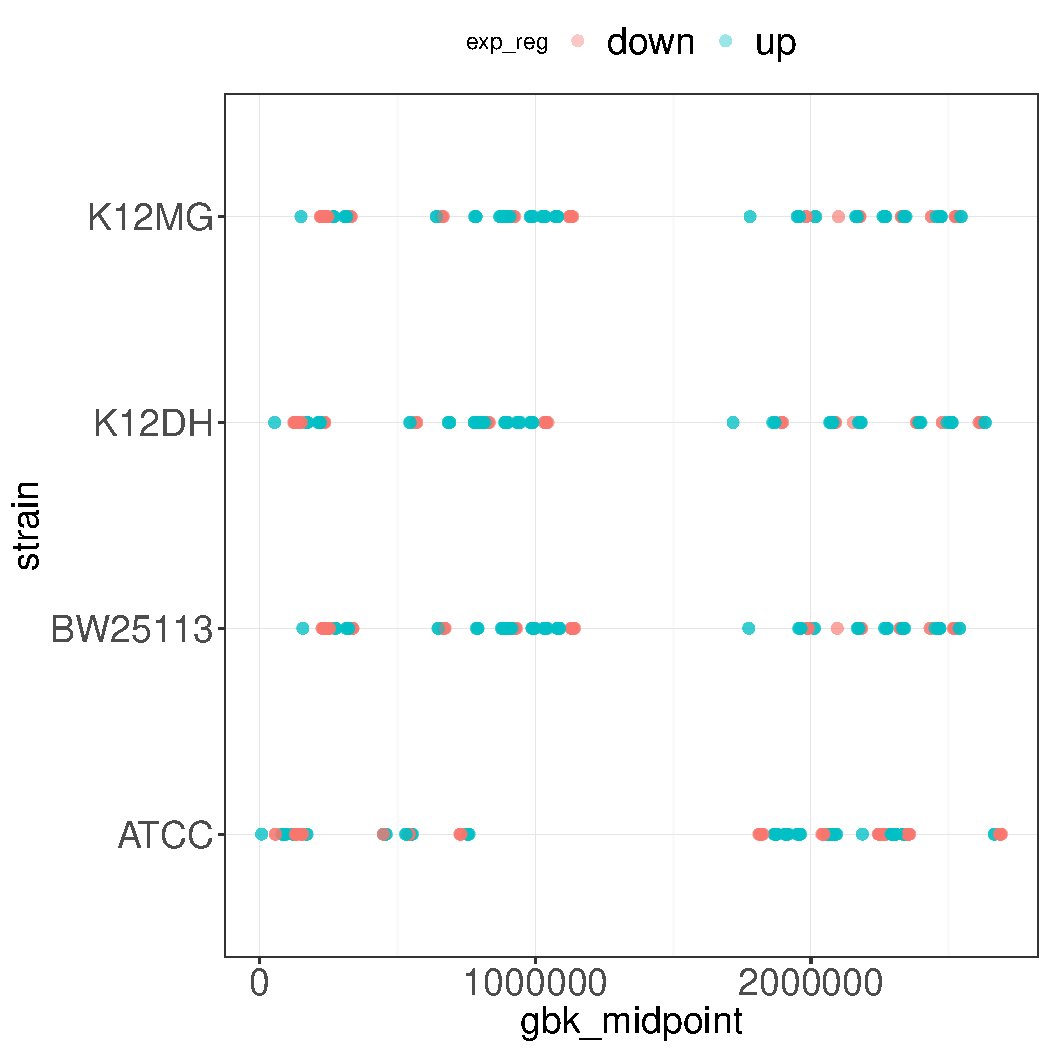
\includegraphics[width=\textwidth]{genome_pos_inversions_attempt1.pdf}
		\caption{\label{fig:inversions_pos_1} An attempt at showing all taxa and the significant inversions (significant $=$ blocks that had a significant difference in gene expression between inverted and non-inverted sequences using wilcox sign-ranked test). The ``up'' and ``down'' simply mean that the sequences that were inverted in that block has significantly higher or lower gene expression than the non-inverted sequences in that block. This up/down was NOT done using DESeq, just a simple wilcox sign-ranked test.}
	\end{center}
\end{figure}

\begin{figure}[h]
	\begin{center}
		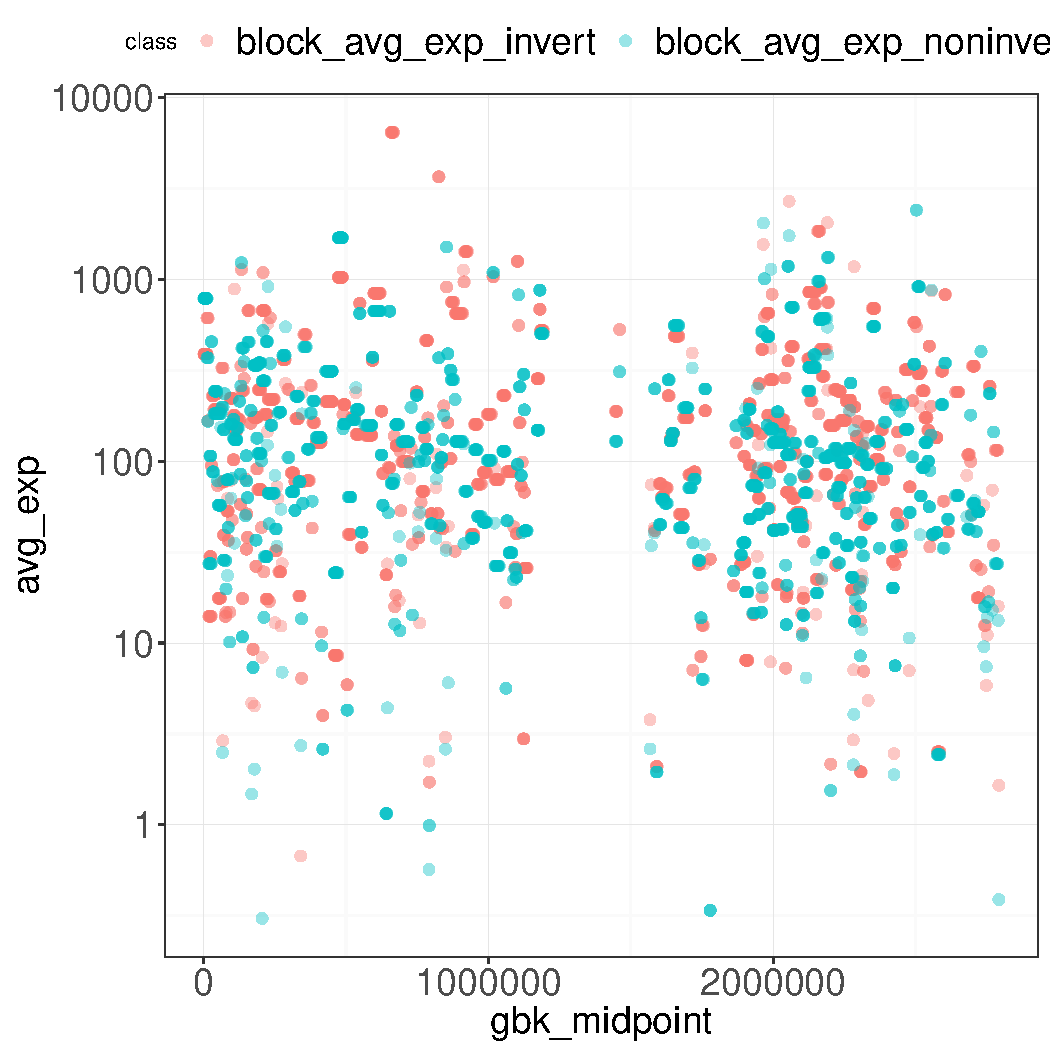
\includegraphics[width=\textwidth]{genome_pos_inversions_k12.pdf}
		\caption{\label{fig:inversions_pos_2} An attempt at showing just the significant inversions (significant $=$ blocks that had a significant difference in gene expression between inverted and non-inverted sequences using wilcox sign-ranked test) using the distance from the origin of \ecol K12 MG655. The ``up'' and ``down'' simply mean that the sequences that were inverted in that block has significantly higher or lower gene expression than the non-inverted sequences in that block. This up/down was NOT done using DESeq, just a simple wilcox sign-ranked test.}
	\end{center}
\end{figure}

\begin{figure}[h]
	\begin{center}
		\includegraphics[width=\textwidth]{genome_pos_inversions_sketch.png}
		\caption{\label{fig:inversions_pos_sketch} A sketch of what I am hoping the position graph would look like. Each inverted region/block would be plotted and the average gene expression of the inverted and non-inverted sequences would be in different colours (green and yellow). Any blocks that had a significant difference in gene expression (significant $=$ blocks that had a significant difference in gene expression between inverted and non-inverted sequences using wilcox sign-ranked test), would be somehow bold in the diagram (red box).}
	\end{center}
\end{figure}

\end{document}
